\documentclass[aspectratio=169,11pt]{beamer}
\usepackage[T1]{fontenc}
\usepackage[utf8]{inputenc}
\usepackage{lmodern}
\usepackage{graphicx}
\usepackage[absolute,overlay]{textpos}

% Compile from presentation/: pdflatex -halt-on-error omnisound-presentation.tex
% Original report figures are included without changing their files.
\definecolor{omniBG}{HTML}{0B0E13}
\definecolor{omniWhite}{HTML}{F4F6F8}
\definecolor{omniMuted}{HTML}{BCC5D0}
\definecolor{omniLime}{HTML}{C4FF5E}
\setbeamercolor{background canvas}{bg=omniBG}
\setbeamercolor{normal text}{fg=omniWhite,bg=omniBG}
\setbeamertemplate{navigation symbols}{}
\setbeamertemplate{headline}{}
\setbeamertemplate{footline}{}
\setbeamertemplate{background}{}
\setbeamersize{text margin left=0mm,text margin right=0mm}
\textblockorigin{0mm}{0mm}
\hypersetup{pdftitle={Omnisound: User-Centred Design of a Unified Audio Interface},
 pdfauthor={Obid Alrhman Aljabi, Yacoub Dawli, Sarshar Chavoshi Rad},
 pdfsubject={DT168G / IU127G, Group 1, 19 October 2026}}

\newcommand{\txt}[5]{%
  \begin{textblock*}{#3mm}(#1mm,#2mm)%
    {\color{omniWhite}\raggedright
    \fontsize{#4pt}{\dimexpr#4pt*6/5\relax}\selectfont
    #5\par}% Keep colour changes inside the stored text box.
  \end{textblock*}}
\newcommand{\pic}[4]{%
  \begin{textblock*}{#3mm}(#1mm,#2mm)%
    \noindent\includegraphics[width=#3mm]{#4}%
  \end{textblock*}}
\newcommand{\heading}[1]{\txt{7}{5}{146}{17.5}{\bfseries #1}}
\newcommand{\footer}{%
  \txt{7}{86.3}{100}{5.5}{\color{omniMuted}OMNISOUND}\txt{145}{86.3}{8}{5.5}{\color{omniMuted}\hfill\insertframenumber/9}}

\begin{document}

% 1. Obid, 0:30
\begin{frame}[plain]
  \txt{10}{15}{140}{36}{\bfseries\color{omniLime}Omnisound}
  \txt{11}{36}{139}{14}{User-Centred Design of a\\Unified Audio Interface}
  \txt{11}{57}{139}{8.7}{\color{omniMuted}Group 1\qquad DT168G / IU127G\qquad 19 October 2026}
  \txt{11}{65}{139}{9.5}{Obid Alrhman Aljabi\\Yacoub Dawli\\Sarshar Chavoshi Rad}
  \footer
\end{frame}

% 2. Obid, 1:30
\begin{frame}[plain]
  \heading{The idea}
  \txt{7}{25}{63}{21}{\bfseries Music\\Podcasts\\Audiobooks}
  \txt{7}{62}{63}{10}{\color{omniLime}One interface, clear categories}
  \txt{78}{24}{75}{11}{\bfseries\color{omniLime}Search}
  \txt{78}{31}{75}{10}{Find audio across the catalogue}
  \txt{78}{43}{75}{11}{\bfseries\color{omniLime}Library}
  \txt{78}{50}{75}{10}{Return to saved content}
  \txt{78}{62}{75}{11}{\bfseries\color{omniLime}Continue Listening}
  \txt{78}{69}{75}{10}{Pick up unfinished audio}
  \txt{7}{78}{146}{8}{\color{omniMuted}An HCI interface prototype with a sample catalogue}
  \footer
\end{frame}

% 3. Obid, 2:30
\begin{frame}[plain]
  \heading{Early designs}
  \txt{7}{19}{85}{8.5}{\bfseries Navigation and content layout}
  \pic{7}{25}{86}{../report/figures/lo-fi/initial-sketch-1.png}
  \txt{98}{17.5}{55}{8.5}{\bfseries Audio categories}
  \pic{98}{23}{55}{../report/figures/lo-fi/initial-sketch-2.png}
  \txt{98}{51}{55}{8.5}{\bfseries Player layout}
  \pic{98}{56.5}{55}{../report/figures/lo-fi/initial-sketch-3.jpg}
  \txt{7}{68}{85}{10.5}{We explored different ways to organise audio before building the prototype.}
  \footer
\end{frame}

% 4. Yacoub, 2:00
\begin{frame}[plain]
  \heading{V1 prototype}
  \txt{7}{18}{86}{8.5}{\bfseries Home}
  \pic{7}{23.5}{86}{../report/figures/v1/home-overview.png}
  \txt{99}{18}{54}{8.5}{\bfseries Search}
  \pic{99}{23.5}{54}{../report/figures/v1/search-focus.png}
  \txt{99}{48.5}{54}{8.5}{\bfseries Library}
  \pic{99}{54}{54}{../report/figures/v1/library-focus.png}
  \txt{7}{69}{86}{10}{Find Weezer, save it, check Library.\\[2pt]Resume an unfinished audiobook.}
  \footer
\end{frame}

% 5. Yacoub, 2:00
\begin{frame}[plain]
  \heading{How we tested}
  \txt{7}{24}{67}{21}{\bfseries\color{omniLime}2 rounds}
  \txt{7}{39}{68}{11}{3 participants per round}
  \txt{7}{49}{68}{8.5}{\color{omniMuted}Different people in each round}
  \txt{7}{62}{68}{11}{Think aloud}
  \txt{7}{71}{68}{9.5}{Task times, routes and comments}
  \txt{83}{24}{70}{12}{\bfseries\color{omniLime}Three tasks each}
  \txt{83}{37}{70}{11}{1. Find and save Weezer,\\\hspace*{4mm}then check Library}
  \txt{83}{54}{70}{11}{2. Resume an unfinished\\\hspace*{4mm}audiobook}
  \txt{83}{71}{70}{11}{3. Browse podcasts}
  \footer
\end{frame}

% 6. Yacoub, 2:00
\begin{frame}[plain]
  \heading{First test findings}
  \txt{7}{22}{52}{30}{\bfseries\color{omniLime}9/9}
  \txt{7}{38}{52}{9.5}{V1 tasks completed}
  \txt{7}{51}{52}{10.5}{\textbf{2 of 3} overlooked\\Continue Listening}
  \txt{7}{68}{52}{10.5}{\textbf{1} brief pause\\at Save}
  \pic{66}{22}{87}{../report/figures/v1/home-comparison.png}
  \footer
\end{frame}

% 7. Sarshar, 2:30
\begin{frame}[plain]
  \heading{What we changed in V2}
  \txt{7}{18}{70}{8.5}{\bfseries V1 Home}
  \txt{83}{18}{70}{8.5}{\bfseries\color{omniLime}V2 Home}
  \pic{7}{23.5}{70}{../report/figures/v1/home-comparison.png}
  \pic{83}{23.5}{70}{../report/figures/v2/home-comparison.png}
  \txt{7}{75}{146}{9.5}{Smaller banner and clearer Continue Listening}
  \txt{7}{81}{146}{8.5}{\color{omniMuted}Stronger Save/Saved states, with the same navigation and categories}
  \footer
\end{frame}

% 8. Sarshar, 2:30
\begin{frame}[plain]
  \heading{Second test results}
  \txt{7}{17.5}{146}{7.5}{\color{omniMuted}Different participants in each round. Observed differences do not prove cause and effect.}
  % The source chart has a transparent page. Keep its original dark labels
  % readable on a white backing without changing or redrawing the chart.
  \begin{textblock*}{104mm}(7mm,23mm)
    \setlength{\fboxsep}{0pt}%
    \colorbox{white}{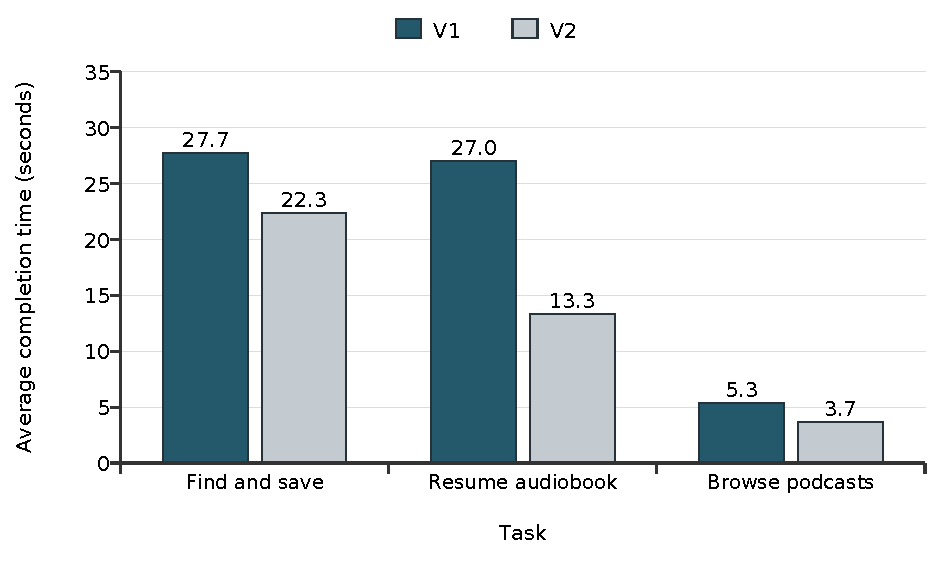
\includegraphics[width=104mm]{../report/figures/results/task-time-comparison.pdf}}
  \end{textblock*}
  \txt{117}{24}{36}{8.5}{Task completion}
  \txt{117}{30}{36}{12}{\bfseries\color{omniLime}V1\enspace 9/9\\V2\enspace 9/9}
  \txt{117}{47.5}{36}{8.5}{Direct Continue\\Listening}
  \txt{117}{57}{36}{10.5}{\bfseries\color{omniLime}V1\enspace 1/3\qquad V2\enspace 3/3}
  \txt{117}{70}{36}{8.5}{Mean resume time}
  \txt{117}{76}{36}{10}{\bfseries\color{omniLime}V1\enspace 27.0\,s\\V2\enspace 13.3\,s}
  \footer
\end{frame}

% 9. Sarshar, 1:30
\begin{frame}[plain]
  \heading{Conclusion}
  \txt{7}{24}{146}{19}{\bfseries\color{omniLime}Testing with users helped us make practical design decisions.}
  \txt{7}{52}{146}{11.5}{A working prototype with connected tasks}
  \txt{7}{63}{146}{11.5}{A focused redesign of the areas users missed}
  \txt{7}{74}{146}{11.5}{Next: more participants and mobile testing}
  \footer
\end{frame}

\end{document}
